\documentclass{article}
\usepackage[utf8]{inputenc}
\setlength{\parindent}{0pt} 
\usepackage{amssymb}
\usepackage{amsmath}
\usepackage{graphicx}
\usepackage{float}
\newcommand{\N}{\mathbb{N}}
\newcommand{\Z}{\mathbb{Z}}
\newcommand{\Q}{\mathbb{Q}}
\newcommand{\R}{\mathbb{R}}
\newcommand{\C}{\mathbb{C}}
\newcommand{\ra}{\longrightarrow}

\title{Homework 2}
\date{}
\author{Julian Lehrer}
\begin{document}
\maketitle
\textbf{Question 1.} Suppose $A$ is symmetric, so $A=A^{T}$. Let $A=Q^{-1}UQ$ be the Schur deomposition of $A$. Then $QAQ^{-1}=QQ^{-1}UQ = IUQ = UQ \implies QAQ^{-1}=UQQ^{-1}=U$. That is, $Q^{-1}AQ = U$, so by definition a is diagonalizable. We now show that $U$ is diagonal. First, note that $U^T = (QAQ^{-1})^T = Q^TA^TQ^{-T} = Q^T A Q^{-T}$ is symmetric. Since $U$ is symmetric, we have that $u_{ij}, i > j = u_{ij} i < j$. But $a_{ij}, i < j = 0$ so $u_{ij} = 0, i \neq j$. Therefore $U$ is diagonal. Finally, we have that $D={\lambda_1,...,\lambda_m}$ since by definition, $A$ is diagonalizable. \\

\textbf{Question 2.} Consider the pertubation of the given system with $c\epsilon > 1$, so we have that 

\begin{equation*}
    \begin{pmatrix}
        1&1\\
        c\epsilon&c
    \end{pmatrix}\begin{pmatrix}
        x\\y
    \end{pmatrix}=
    \begin{pmatrix}
        2c\\c
    \end{pmatrix}
\end{equation*}

Then solving via Gaussian elimination with partial pivoting, we have that 
\begin{align*}
    &\begin{pmatrix}
        1&1\\
        c\epsilon&c
    \end{pmatrix}\begin{pmatrix}
        x\\y
    \end{pmatrix}=
    \begin{pmatrix}
        2c\\c
    \end{pmatrix}=\\
    &\begin{pmatrix}
        c\epsilon&c\\
        1&1
    \end{pmatrix}\begin{pmatrix}
        x\\y
    \end{pmatrix}=
    \begin{pmatrix}
        c\\2c
    \end{pmatrix}=\\
    &\begin{pmatrix}
        c\epsilon & c\\
        0 &1-\frac{1}{\epsilon}
    \end{pmatrix}\begin{pmatrix}
        x\\y
    \end{pmatrix} = 
    \begin{pmatrix}
        c\\
        2c-1/\epsilon
    \end{pmatrix}=\\
\end{align*}
Therefore, we have that
\begin{equation*}
    y=\frac{2c-1/\epsilon}{1-1/\epsilon}
\end{equation*}
And the first equation gives us that  
\begin{align*}
    (c\epsilon)x+cy&=c \\
    \left(c\epsilon\right)x+c\left(\frac{2c-1/\epsilon}{1-1/\epsilon}\right) &= c\\
    \left(c\epsilon\right)x &= c\left(1-\frac{2c-1/\epsilon}{1-1/\epsilon}\right)\\
    &x=\frac{1}{\epsilon}\left(1-\frac{2c-1/\epsilon}{1-1/\epsilon}\right)
\end{align*}
Now consider the case if $c \epsilon \leq \epsilon_{\text{mach}}$. We'll have that $x=0$.\\

Next, consider the implicit pivoting algorithm, where we first divide each term of the augmented matrix (i.e. both the LHS and RHS) by the largest absolute value in each row. This gives us the system 
\begin{equation*}
    \begin{pmatrix}
        \frac{1}{2c}&\frac{1}{2c}\\
        \epsilon & 1
    \end{pmatrix}\begin{pmatrix}
        x\\y
    \end{pmatrix}=
    \begin{pmatrix}
        1\\1
    \end{pmatrix}
\end{equation*}
Using Gaussian elimination, we obtain that 
\begin{align*}
    &\begin{pmatrix}
        \frac{1}{2c}&\frac{1}{2c}\\
        \epsilon & 1
    \end{pmatrix}\begin{pmatrix}
        x\\y
    \end{pmatrix}=
    \begin{pmatrix}
        1\\1
    \end{pmatrix}= \\
    &\begin{pmatrix}
        \frac{1}{2c}&\frac{1}{2c}\\
        0&1-\epsilon
    \end{pmatrix}\begin{pmatrix}
        x\\y
    \end{pmatrix}=
    \begin{pmatrix}
        1\\
        1-2c\epsilon
    \end{pmatrix} 
\end{align*}
So we have that 
\begin{equation*}
    y(1-\epsilon) =1-2c\epsilon \implies y = \frac{1-2c\epsilon}{1-\epsilon}
\end{equation*}
Substituting this into our equation for $x$, we obtain that 
\begin{align*}
    \frac{x}{2c} + \frac{\left(\frac{1-2c\epsilon}{1-\epsilon}\right)}{2c} &= 1\\
    \frac{x}{2c} + \frac{1-2c\epsilon}{2c(1-\epsilon)} &= 1 \\
    \frac{x}{2c} &= 1-\frac{1-2c\epsilon}{2c(1-\epsilon)}\\
    x &= 2c - \frac{1-2c\epsilon}{1-\epsilon}
\end{align*}

We can see that in our first attempt via Gaussian elimination with partial pivoting, there are numerical issues in the elimination step of row two. Since we are dividing by $1/\epsilon$, the bottom right value may have numerical issues. If we manage to solve for $y$ okay, $x$ will be unstable since it's value is multiplied by $1/\epsilon$ as well. The implicit pivoting algorithm is better in this sense. Since we substract epsilon in the elimination step, there should be no numerical issues. Indeed, solving for $y$ should also be stable, and since $x$ is a simple subsitution it should be okay as well. Therefore, the implicit pivoting algorithm solves numerical instability in this problem.\\
% Since $1/\epsilon = 0$. To alleviate this numerical issue, we can use implicit pivoting, where each row of the matrix is scaled by the largest absolute value in its entries. Therefore, we would have the system 
% \begin{equation*}
%     \begin{pmatrix}
%         1/2 & 1/2\\
%         \epsilon & 1
%     \end{pmatrix}\begin{pmatrix}
%         x\\y
%     \end{pmatrix}=
%     \begin{pmatrix}
%         1\\ 1
%     \end{pmatrix}
% \end{equation*}
% Which we previously showed was numerically stable with partial pivoting (see pg. 37 of chapter 2 notes).\\

\textbf{Question 3.} Let $A$ be symmetric and positive-definite, so $x^*Ax > 0$. First, note that since $A$ is symmetrics, $a_{ii}=a_{ii}^*$, so $a_{ii}$ is real since the only way a complex number can be equal to it's conjugate transpose is if the imaginary part is zero. Then let $x=e_i$, the $i$th basis vector. So $e_i^* A e_i = e_i^T A e_i = a_{ii} > 0$, therefore the diagonals are both real and strictly postive. \\

\textbf{Question 4.} 
\begin{itemize}
    \item[a.] We have that \begin{align*}
        &\begin{pmatrix}
            I&0\\
            -A_{21}A^{-1}_{11}&I
        \end{pmatrix}
        \begin{pmatrix}
            A_{11}&A_{12}\\
            A_{21}&A{22}
        \end{pmatrix}\\
        &=
        \begin{pmatrix}
            IA_{11}+0A_{12}&IA_{12}+0A_{22}\\
            -A_{21}A^{-1}_{11}A_{11}+A_{21}&-A_{12}A_{21}A^{-1}A_{11}+A_{22}
        \end{pmatrix}\\
        &= 
        \begin{pmatrix}
            A_{11}&A_{12}\\
            A_{21}-A_{21}(A^{-1}_{11}A_{11})&A_{22}-A_{12}A_{21}A^{-1}A_{11}
        \end{pmatrix}\\
        &= \begin{pmatrix}
            A_{11}&A_{12}\\
            0&A_{22}-A_{12}A_{21}A^{-1}A_{11}
        \end{pmatrix}
    \end{align*}
    \item[b.] We want that the first block matrix of the second row $A_{21}$ is eliminated. Therefore, we must multiple the first row by $A_{11}^{-1}$ so the first block entry is $A_{11}^{-1}A_{11}=I$. Then we also multiply by $A_{21}$, so upon subtraction of row 1 from row 2 that $A_{21}=0$. Therefore, we subtract by $[A_{21}A_{11}^{-1}A_{11} \ \ A_{21}A^{-1}_{11}A_{12}]$ and obtain
    \begin{equation*}
        \begin{pmatrix}
            A_{11} & C\\
            0 & A_{22} - A_{21}A^{-1}_{11}A_{12}
        \end{pmatrix}
    \end{equation*} 
    as desired. 
\end{itemize}


\textbf{Question 5.}
\begin{itemize}
    \item[a.] Let $A=A_1+iA_2$, $b=b_1+ib_2$ and $x=x_1+ix_2$. Then consider the system $(A_1+iA_2)(x_1+ix_2)=b_1+ib_2$. Let $x=(x_1,...,x_n)$ be our solution vector where $x_i=\alpha_i + i \beta_i$. Then consider $x'=(x_1,...,x_{n}, x_{n+1},...,x_{2n})$, where the elements $x_{n+1},...,x_{2n}$ correspond to the $\beta_i, i=1,...,n$. And similarly for $b'$. Then we have that the system 
    \begin{equation*}
        [A_1 A_2]x' = b'
    \end{equation*} 
    Is a system of a $2n \times 2n$ matrix with vectors $x$ and $b$ of length $2n$. 
    \item[b.] Suppose our Gaussian elimination for an $n\times n$ system takes $n$ steps. Note that since complex numbers $x_1 = \alpha_1 + i\beta_1, x_2=\alpha_2 + i \beta_2$, then $x_1 x_2$ actually has a total of $4$ multiplication operations, not one. The exact computational cost for the real valued system is $16n^3/3=O(n^3)$ operations, where as the big-O computational cost of the complex system will be $O(n^4)$. Therefore, we have that for large $n$, it is better to use the real-valued equivalent of the system. 
\end{itemize}

\textbf{Section 2, question 5.} Here, we want our points to all sit in some plane whose coefficients we must define. Therefore, consider the equation of a plane, $ax+by+cz+d=0$. With the three points we currently have, this gives us an underdetermined system of equations. However, by using a new vector on the plane given by $(A-B) = (4, 0, -2)$, we obtain the system of equations 
\begin{align*}
    a+2b+3c+d&=0\\
    -3a+2b+5c+d&=0\\
    \pi a+eb-\sqrt{2}c + d&=0\\
    4a + 0b +-2c+d &=0
\end{align*}

Which gives the system 
\begin{equation*}
    \begin{pmatrix}
        1&1&3&1\\
        -3&2&5&1\\
        \pi&e&-\sqrt{2}&1\\
        4&0&-2&1
    \end{pmatrix}\begin{pmatrix}
        a\\b\\c\\d
    \end{pmatrix} = \begin{pmatrix}
        0\\0\\0\\0
    \end{pmatrix}
\end{equation*}
Which are contained in the plane given by  
\begin{equation*}
    (4-2e)x+(-14-4\sqrt{2}+2\pi)y + (8-4e)z+8\sqrt{2}+14e-4\pi = 0
\end{equation*} 
Which is plotted numerically in plot.py. The visualization can be seen below. 

\begin{figure}[H]
    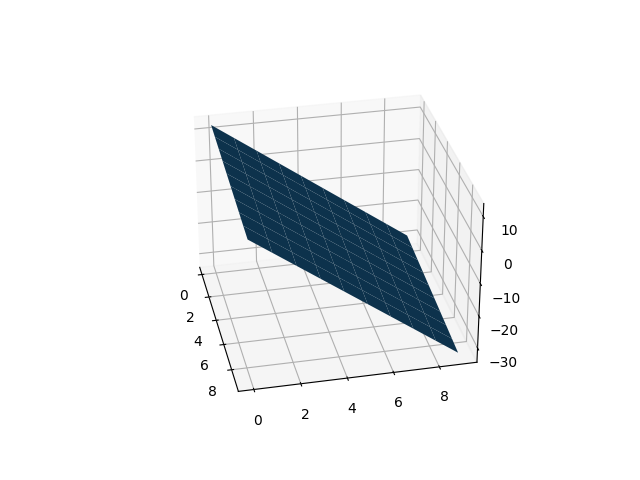
\includegraphics[scale=0.5]{code/plane.png}
\end{figure}

\end{document}
